\section{Naleśniczki bananowe}
\bigskip
\small
\begin{minipage}{0.45\textwidth}
    \noindent \textbf{Czas:} 20 minut \\
    \textbf{Poziom trudności:} łatwy
\end{minipage}
\begin{minipage}{0.45\textwidth}
    \noindent \textbf{Ilość sprzątania:} średnia \\
    \textbf{Wymagany mysi sprzęt:} -
\end{minipage}
\normalsize
\vspace{0.5cm}

\begin{multicols}{2}

\subsection*{Składniki} \begin{itemize} \item 2 dojrzałe banany \item 2 jajka \item 2 duże łyżki jogurtu greckiego \item 2 łyżki cukru lub miodu (opcjonalnie) \item szklanka mąki \item 2 łyżeczki proszku do pieczenia \item olej do smażenia \end{itemize}

\columnbreak

\begin{figure}[H] \centering
\fbox{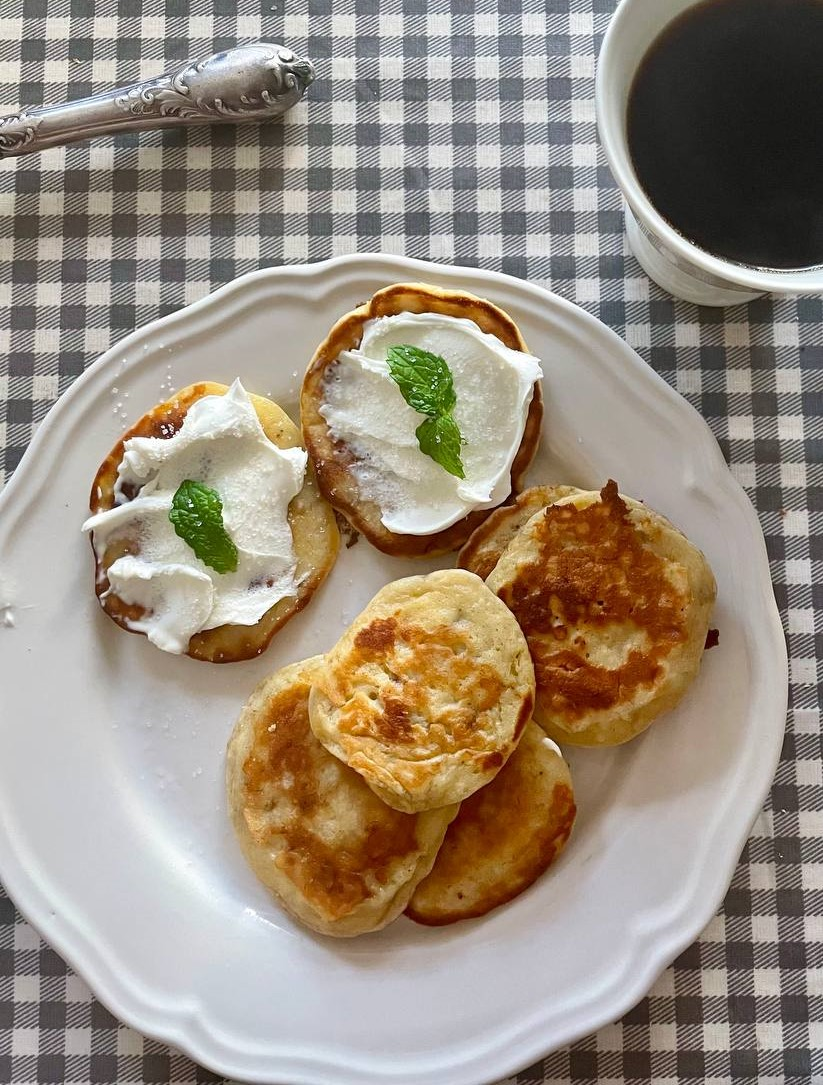
\includegraphics[width=0.35\textwidth]{images/nalesniczki.jpg}}
\end{figure}

\end{multicols}

\vspace{0.5cm}

\subsection*{Instruktaż} \begin{enumerate} \item Banany rozgnieść widelcem na papkę, wbić jajka, ewentualnie dodać cukier, jogurt i wymieszać. \item Mąkę połączoną z proszkiem do pieczenia dodawać powoli i stopniowo, jednocześnie mieszając, aż do uzyskania jednolitej mikstury o odpowiedniej konsystencji. \item Patelnię rozgrzać na średnim ogniu, wlać niewielką ilość oleju i zaczekać około 2 minuty, aż nabierze temperatury. Zmniejszyć ogień i wlać po łyżce ciasta na każdego naleśniczka. Gdy krawędzie zaczną się ścinać lub pojawią się na nich bąbelki (około 3-5 minut), ostrożnie przewrócić na drugą stronę i smażyć, aż się zarumienią. \end{enumerate}

\vspace{0.5cm}

\small \subsection*{Propozycja podania} Z bitą śmietaną, z cukrem pudrem, z dżemem, z jogurtem, z masłem orzechowym, z kremem czekoladowym, z owocami.

\vspace{0.3cm}

\subsection*{Dodatkowe uwagi} W zależności od tego, jak miękkie i dojrzałe są banany oraz jak duże są jajka, mieszanka może być zbyt wodnista lub zbyt gęsta - w takim wypadku należy dodać albo odrobinę więcej mąki, żeby ciasto zagęścić, albo niewielką ilość wody/mleka, aby stało się bardziej luźne.\ Ciasto można również urozmaicić poprzez dodanie do mąki odrobiny cynamonu, przyprawy do piernika, cukru wanilinowego lub kawałków czekolady.

\newpage
